\chapter{Combinations of Run 1 searches for invisibly decaying Higgs bosons}
\label{chap:comb}
Whilst the \ac{VBF} production mode offers the best sensitivity to invisibly decaying Higgs bosons, the limit on \BRinv can be improved by taking into account searches performed using other production channels. According to the $CL_{S}$ method described in \SectionRef{sec:stats} multiple searches can be combined by constructing a likelihood, according to \EquationRef{eq:likelihood}. Combinations of the \ac{VBF} analyses with the other channels are described in sections \ref{sec:combotherchannels} to \ref{sec:combparked}. 

%CHECK PLOT AXIS LABEL SIZES AND THAT LEGEND TERMS ARE STANDARD OR IN TEXT

\section{Searches in other channels}
\label{sec:combotherchannels}
%Refer back to theory to introduce ZH and ggH searches
As described in \SectionRef{sec:higprod}, after \ac{VBF} the next most sensitive production modes to invisible Higgs boson decays are \ac{ggH} and \ac{VH}. \ac{VH} has a much lower production rate than \ac{VBF} (approximately 4 times less for a 125 \GeV Higgs boson). Compensating for this low cross-section, several of the final states in \ac{VH} production, particularly \ac{ZH}, give very clean signatures which are easy to identify. Gluon fusion has a much higher rate than \ac{VBF}, but in most cases the resulting Higgs boson is created alone so there are no visible particles in the final state. However, one or more jets can result from \ac{ISR} allowing this channel to also be used. 

In addition to the \ac{VBF} analyses, three invisibly decaying Higgs boson searches were carried out by CMS during Run 1. Two of these searches specifically targeted the \ac{ZH} production mode, one searching for events where the \PZ boson decayed to two leptons (the Z$(\ell\ell)$H search) and another where it decayed to two b quarks (the Z$(b\bar{b})$H search). The third ``monojet'' search targeted events with one or more jets that are not \ac{VBF}-like and included categories targeting \ac{ggH} with \ac{ISR}, and \ac{VH} production where the vector boson decays hadronically. The fraction of the signal expected to come from each production mode in each category of each search along with the integrated luminosity used is given in \TableRef{tab:analysissummary}. The limits from each search alone on \BRinv for a 125 \GeV Higgs boson are given in \TableRef{tab:combinedlimits}.

When combining limits from separate analyses it is important that the event selections are mutually exclusive. A brief description of the event selection used in each of the non-\ac{VBF} invisibly decaying Higgs searches is therefore given in the following subsections. It is also important when constructing the overall likelihood function to understand which uncertainties are correlated between analyses and which are not. The correlated uncertainties are discussed in Sections \ref{sec:combprompt} and \ref{sec:combparked}. 

%signal fraction table
\begin{table}
\caption{Summary of the analyses included in the combination. The first column is the name of the analysis. The second and third columns give the integrated luminosity of the 7 and 8 TeV data sets used by each analysis. The fourth column contains the names of the categories in each analysis and the fifth column gives the proportion of signal events expected to come from each Higgs boson production mode.}
           \begin{center}
           \begin{tabular}{lccc}
           \hline
           \multirow{2}{*}{Analysis} & Luminosity (\invfb) &\multirow{2}{*}{Category} & Expected signal \\
           \cline{2-2}
           & 8 TeV (7 TeV) & & composition \\
           \hline
           \hline
           VBF prompt data &  19.5 & 2-jet VBF & 94\% VBF, 6\% ggH \\
           \hline
           VBF parked data &  19.2 & 2-jet VBF & 92\% VBF, 8\% ggH \\
           \hline
           \multirow{6}{*}{Monojet} & \multirow{6}{*}{19.7} & Monojet & 70\% ggH, 20\% VBF, \\
            & & & 6\% WH, 3\% ZH \\
            & & unresolved & 47\% WH, 25\% ggH, \\
            & & &  23\% ZH, 5\% VBF \\
            & & resolved & 39\% ggH, 32\% WH, \\
            & & &  18\% ZH, 11\% VBF \\
           \hline
           \multirow{4}{*}{Z$(\ell\ell)$H} & \multirow{4}{*}{19.7 (4.9)} & \Pep\Pem - 0-jet & 100\% ZH \\
            & & \Pep\Pem - 1-jet &  100\% ZH\\
            & & \Pgmp\Pgmm - 0-jet &  100\% ZH\\
            & & \Pgmp\Pgmm - 1-jet &  100\% ZH\\
           \hline
           \multirow{3}{*}{Z$(b\bar{b})$H} & \multirow{3}{*}{18.9} & 2-b-jet - low \MET & 100\% ZH \\
            & & 2-b-jet - medium \MET &  100\% ZH\\
            & & 2-b-jet - high \MET &  100\% ZH\\
           \hline
           \end{tabular}
           \end{center}
           \label{tab:analysissummary}
\end{table}

%individual limits
\begin{table}
\begin{center}
\caption{Summary of 95\% CL upper limits on $\frac{\sigma}{\sigma_{SM}}\cdot$\BRinv for a 125 \GeV Higgs boson obtained from each individual search contributing to the combinations described in this section~\cite{Chatrchyan:2014tja,CMS-PAS-HIG-15-012}.}
        \begin{tabular}{lc}
                \hline
                \hline
                \multirow{2}{*}{Channel}        & Observed (expected) upper limits \\
                                                                                & on $\frac{\sigma}{\sigma_{SM}}\cdot$ \BRinv (\%)\\
                \hline
                \hline
                VBF prompt data               & 65 (49) \\
                VBF parked data               & 57 (40) \\
                Z$(\ell\ell)$H              & 84 (87) \\
                Z$(b\bar{b})$H              & 192 (198) \\ 
                Monojet                       & 54 (62) \\
                \hline
                \hline
        \end{tabular}
        \label{tab:combinedlimits}
\end{center}
\end{table}


\subsection{Z$(\ell\ell)$H$\rightarrow$invisible selection}
\label{sec:zllh}
%sel
The Z$(\ell\ell$)H search is described in Ref.~\cite{CMS-PAS-HIG-13-018}. The analysis selection required two tight, oppositely charged, same flavour leptons (either electrons or muons) both with \pt$>20$ \GeV, with invariant mass compatible with the \PZ boson, no further leptons and large \MET. Events containing two or more jets with \pt$>30$ \GeV are rejected to reduce the $\PZ+$jets background. 

To reduce backgrounds, in events with a single jet, that jet was required not to be identified using the \ac{CSV} algorithm (described in \SectionRef{sec:parkedtop}) as a b-jet. Also, requirements were made on the azimuthal angular separation and \pt balance between the \MET and the dilepton system. In addition to this signal region, control regions, which differ from the signal region in that the lepton system is not compatible with a \PZ boson decay, were used for background estimation. As events with two or more jets were always vetoed there is no overlap with the events selected in the \ac{VBF} and Z$(b\bar{b})$H analyses (where two jets with \pt$>30$ \GeV are required). 

\subsection{Z$(b\bar{b})$H$\rightarrow$invisible selection}
\label{sec:zbbh}
%sel
The Z$(b\bar{b})$H search is described in Ref.~\cite{CMS-PAS-HIG-13-028}. The analysis selection required two jets tagged by the \ac{CSV} algorithm as originating from b-quarks, large \MET, and no reconstructed electrons or muons. The di-b-jet system was required to have high \pt, but low invariant mass (less than 250 \GeV). The dijet mass cut ensured there was no overlap with either of the \ac{VBF} analyses. The main background to the analysis was from \ac{QCD} multijet processes as in the \ac{VBF} analysis. Similarly to the selection in the \ac{VBF} parked data analysis this background was reduced using requirements on \jetmetdphi and \METsig. The neutral component of the \MET was also required to be aligned with the charged component in $\phi$. The signal region was separated into three categories with with low, medium and high \MET and control regions where the signal region selections are relaxed or inverted are used to estimate the remaining backgrounds.

\subsection{Monojet selection}
\label{sec:monojet}
%sel
The ``monojet'' search, is described in Ref.~\cite{CMS-PAS-EXO-12-055}. This analysis selected events with large \MET, one or more high-\pt jets, and no reconstructed electrons or muons. To separate events due to \ac{ggH} production with \ac{ISR} from those due to \ac{VH} production where the vector boson decays hadronically, events were classified into three signal categories. The categorisation was sequential, i.e. if an event passed the requirements for the first category it was not considered for the second etc. 

The first category targeted ``unresolved'' vector bosons where the high \pt of the vector boson caused its decay products to be very close together. These unresolved vector bosons were identified by searching for so-called ``fat'' jets with substructure with \pt$>200$ \GeV, (described in detail in Ref.~\cite{CMS-PAS-EXO-12-055}). One additional normal jet was allowed in this category as long as it was within 2 in $\phi$ of the fat jet.

The second category was the resolved category where the vector boson had lower \pt and its decay products could be identified as two separate normal jets. These jets were required to have an invariant mass between 60 and 110 \GeV. This range overlaps with the range used in the Z$(b\bar{b})$H analysis regions, leading to a non-negligible number of events passing the selection for both analyses. The resolved category was therefore not used in any combinations.

The third category was the ``monojet'' category. Events in this category were required to have one jet with \pt$>150$ \GeV. One additional jet within 2 in $\phi$ of the first jet was allowed to be present, with further jets causing the event to be vetoed. Control regions, which differ from the above categories by the presence of one or more leptons or photons, were used to estimate the background.

The category definitions above are not orthogonal to the \ac{VBF} analysis. To remedy this any events passing the \ac{VBF} parked data analysis selection were vetoed. This veto removed less than 4\% of the expected signal events in the monojet category and none of the signal events expected in the resolved category. As the monojet analysis was performed in 2015, after the parked data \ac{VBF} analysis had been performed, the monojet analysis was not combined with the prompt analysis, so no overlap veto between these two analyses was necessary.

The lepton veto present in all three signal categories means there is no overlap of any of the three categories with the Z$(\ell\ell)$H analysis. Some of the control regions do overlap slightly with categories in the Z$(\ell\ell)$H search. However, these overlaps are very small due to the very high jet \pt cut present in the monojet search. In addition to the Z$(b\bar{b})$H search overlapping with the resolved category, there are also overlaps between the Z$(b\bar{b})$H search and the  unresolved and monojet categories. However, very few events in the Z$(b\bar{b})$H search have jets with \pt$>150$ \GeV, so these overlaps were considered negligible.

\section{Combination with prompt data VBF search}
\label{sec:combprompt}
%Present combination
The first combination that was performed was between the analyses that were completed in 2013, the two ZH searches and the prompt data \ac{VBF} search. As has been described above, these analyses do not overlap. However, as the objects used in all three analyses are very similar, several of the systematic uncertainties are correlated. The full list of correlated uncertainties, and the analyses they affect, are given, in decreasing order of the change in the expected limit on \BRinv for a 125 \GeV Higgs boson as a result of removing the uncertainty, in \TableRef{tab:promptcorrs}. The method for determining the jet energy in the Z$(b\bar{b})$H analysis, involving a regression technique, is very different from that used in the other two analyses~\cite{CMS-PAS-HIG-13-028}. The jet uncertainties are therefore correlated between the Z$(\ell\ell)$H and \ac{VBF} searches, but not the Z$(b\bar{b})$H analysis.

%correlation decisions
\begin{table}
  \caption{Uncertainties correlated between the \ac{VBF} prompt data, Z$(\ell\ell)$H and Z$(b\bar{b})$H searches and the analyses they affect. Also quoted is the relative change in the expected limit on \BRinv on removing each uncertainty from the analysis.}
  \label{tab:promptcorrs}
  \begin{tabular}{lcc}
    \hline
    \hline
    Uncertainty & Analyses affected & $\frac{\Delta(\rm(limit))}{\rm{limit}}$ on removal \\
    \hline
    \ac{JES} & VBF, Z($\ell\ell$)H & -0.13 \\
    PDFs & VBF, Z($b\bar{b}$), Z($\ell\ell$)H & -10 \\
    QCD scale & VBF, Z($b\bar{b}$), Z($\ell\ell$)H & -0.04\\
    Luminosity & VBF, Z($b\bar{b}$)H, Z($\ell\ell$)H & -0.02\\
    \ac{JER} & VBF, Z($\ell\ell$)H & $<$0.01\\
    \ac{UES} & VBF, Z($b\bar{b}$)H, Z($\ell\ell$)H & $<$0.01\\
    Lepton efficiency & VBF, Z($\ell\ell$)H & $<$0.01\\
    \hline
    \hline
  \end{tabular}
\end{table}

%interpolation
None of the analyses saw any significant excess of events, so limits were set using the asymptotic $CL_{S}$ procedure described in \SectionRef{sec:stats} for several Higgs boson mass hypotheses. The Higgs boson masses for which the three analyses have generated \ac{MC} samples are not all the same. Between 115 and 145 \GeV the two ZH analyses have samples for the same masses. Limits from the combination of these two analyses were obtained in this range and can be seen in \FigureRef{fig:zhcomb}. Assuming \ac{SM} Higgs boson production and acceptance the 95\% \ac{CL} observed (expected) limit on \BRinv for a 125 \GeV Higgs boson is found to be 0.81 (0.83).

The mass points available in the \ac{VBF} and ZH analyses are quite different. The selection efficiency for \ac{VBF} and \ac{ggH} signal events in the \ac{VBF} analysis was interpolated between the available mass points (these ranged from 110 to 400 \GeV). Multiplying the interpolated efficiencies for a mass hypothesis by the corresponding Higgs boson production cross-section gives a signal yield estimate for that mass. 

In order to combine limits from multiple production channels it is also necessary to make an assumption about the relative cross-section of these two production mechanisms. Assuming the \ac{SM} production cross-sections, a combination was performed between all three analyses in the mass range 115 to 145 \GeV. The results of this combination can be seen in \FigureRef{fig:promptcomb}. The 95\% \ac{CL} observed (expected) limit on \BRinv for a 125 \GeV Higgs boson was found to be 0.58 (0.44).

Whilst the Z$(b\bar{b})$H search has no \ac{MC} samples available for Higgs boson masses above 145 \GeV, the Z$(\ell\ell)$H search has samples up to 300 \GeV. The \ac{VBF} and Z$(\ell\ell)$H searches were therefore combined in the mass range 115 to 300 \GeV. The results of this combination are shown in \FigureRef{fig:promptcombhighmass}. It can be seen that there is an approximately one sigma excess for all values of the Higgs boson mass. This excess is driven by the \ac{VBF} channel, which also sees a one sigma excess (as shown in \FigureRef{fig:promptlimits}) which is 100\% correlated across all Higgs boson mass hypotheses. The observed excess is therefore not significant.

\begin{figure}
  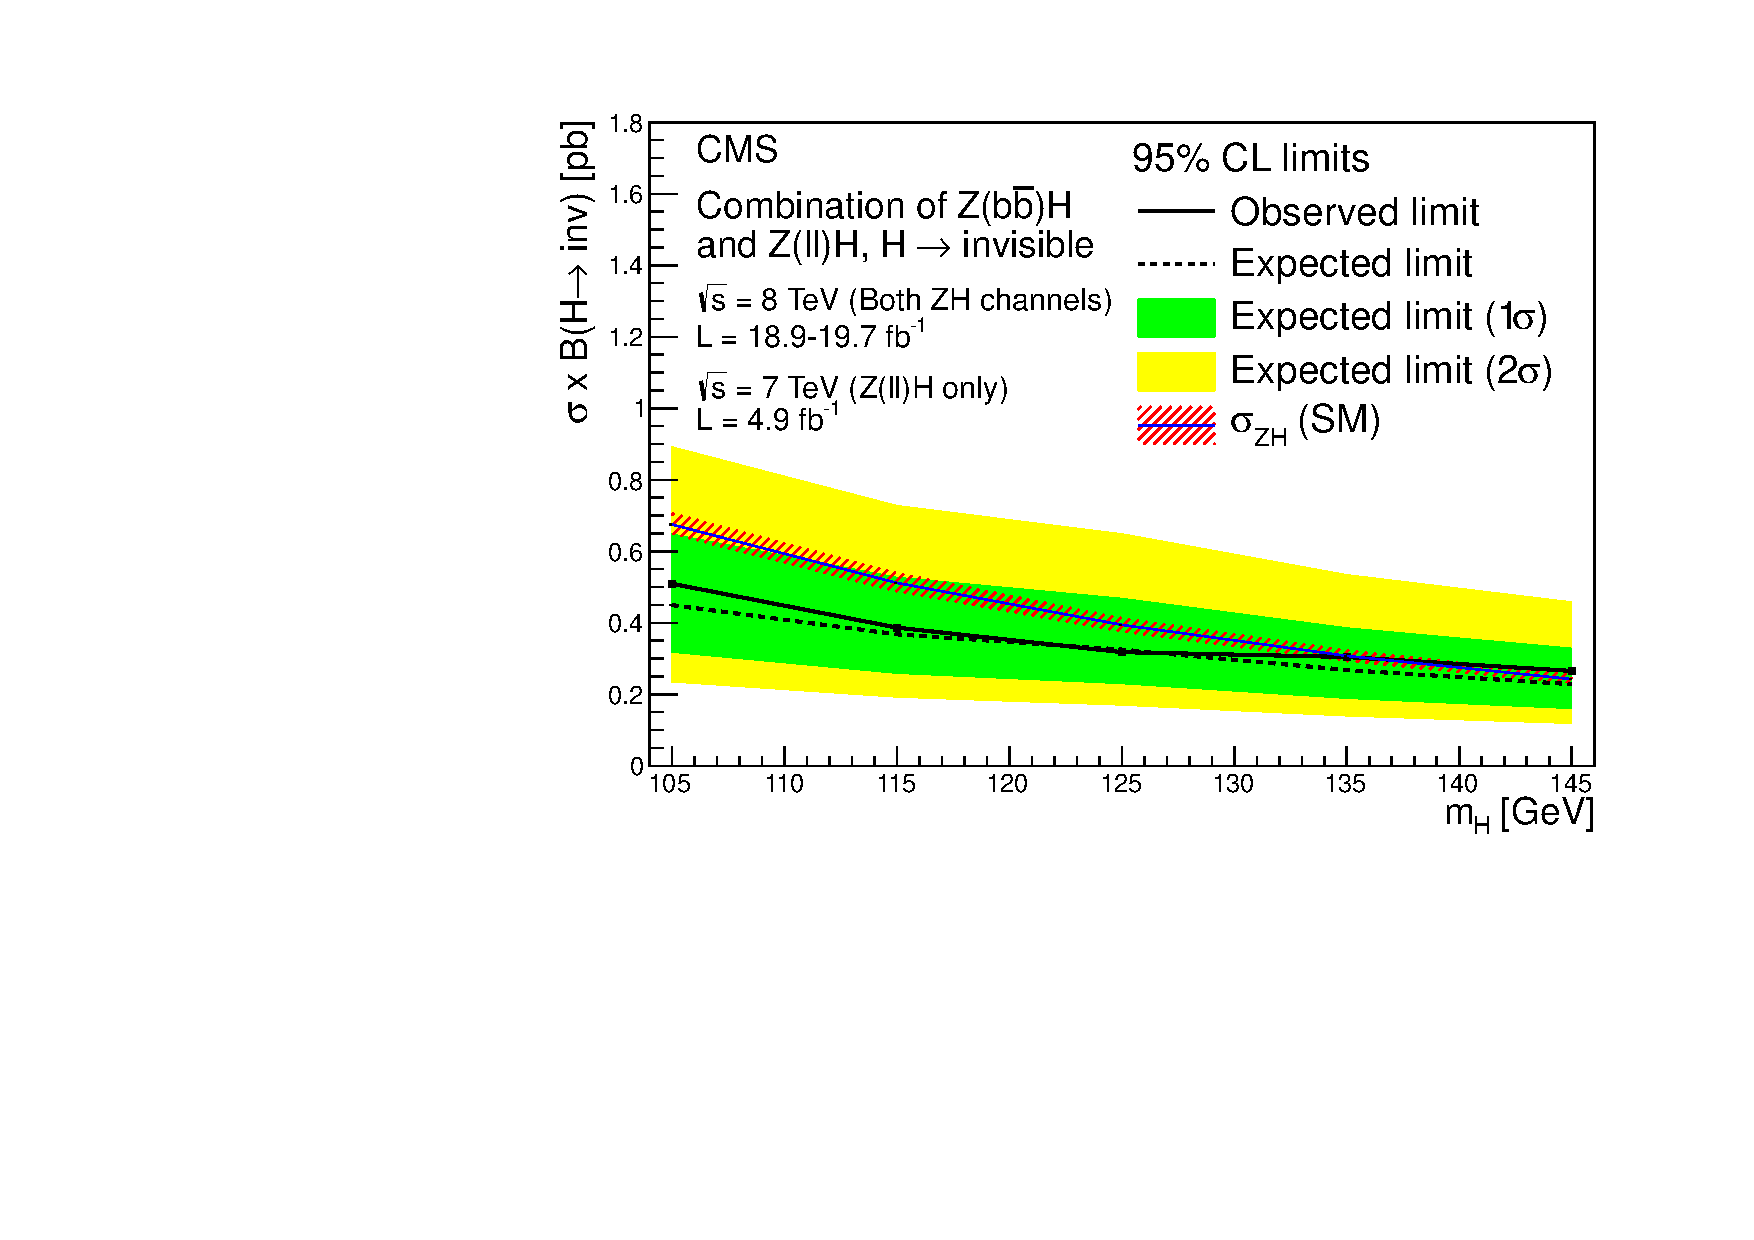
\includegraphics[width=.65\largefigwidth]{plots/prompt/HIG-13-30-figs/zhxslimit.pdf}
  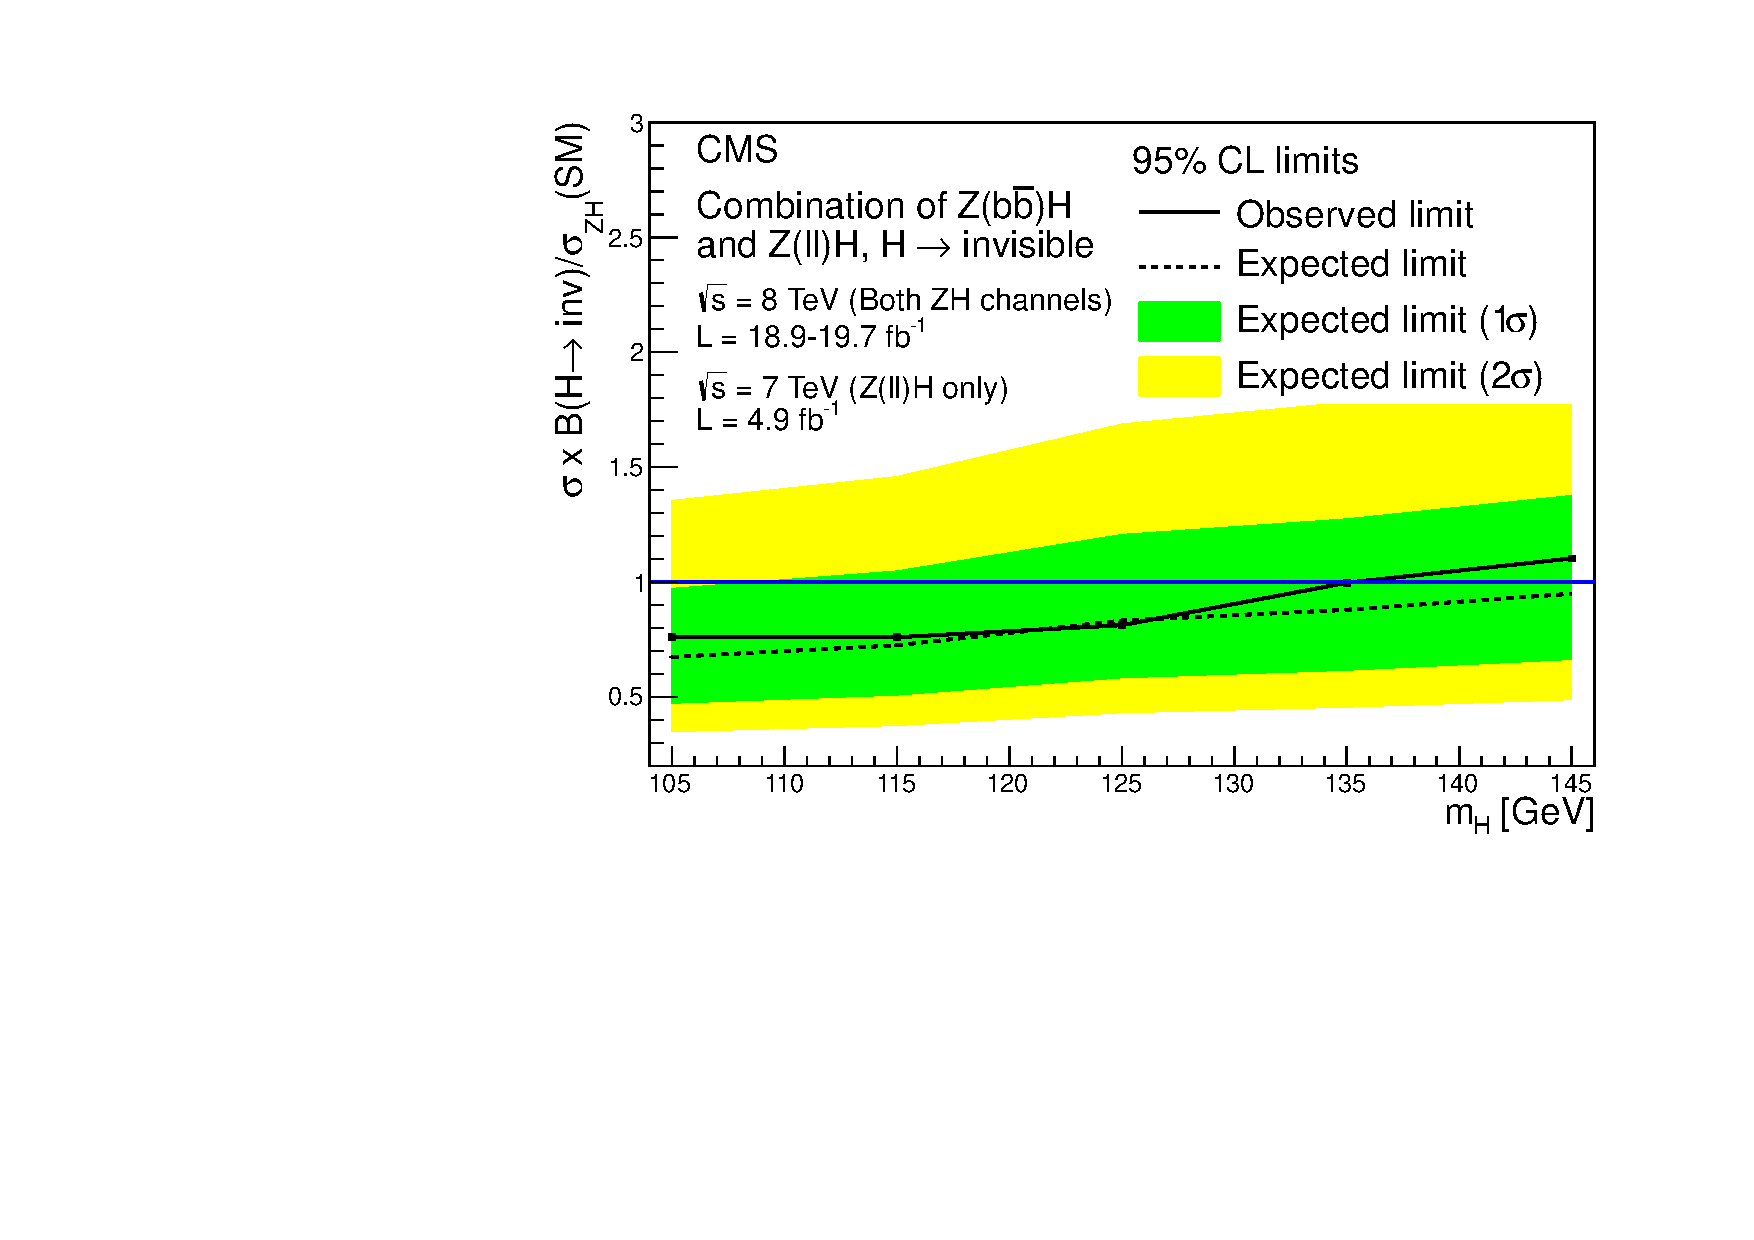
\includegraphics[width=.65\largefigwidth]{plots/prompt/HIG-13-30-figs/zhlimit.pdf}
  \caption{Expected and observed 95\% \ac{CL} upper limits on the \ac{ZH} $\sigma\times\BRinv$ in \pb (a) and normalised to the SM \ac{VBF} Higgs boson production cross-section (b) obtained from the combination of the Z$(\ell\ell)$H and Z$(b\bar{b})$H searches. The green and yellow bands indicate the 68\% and 95\% confidence intervals on the expected limit respectively~\cite{Chatrchyan:2014tja}.}
  \label{fig:zhcomb}
\end{figure}

\begin{figure}
  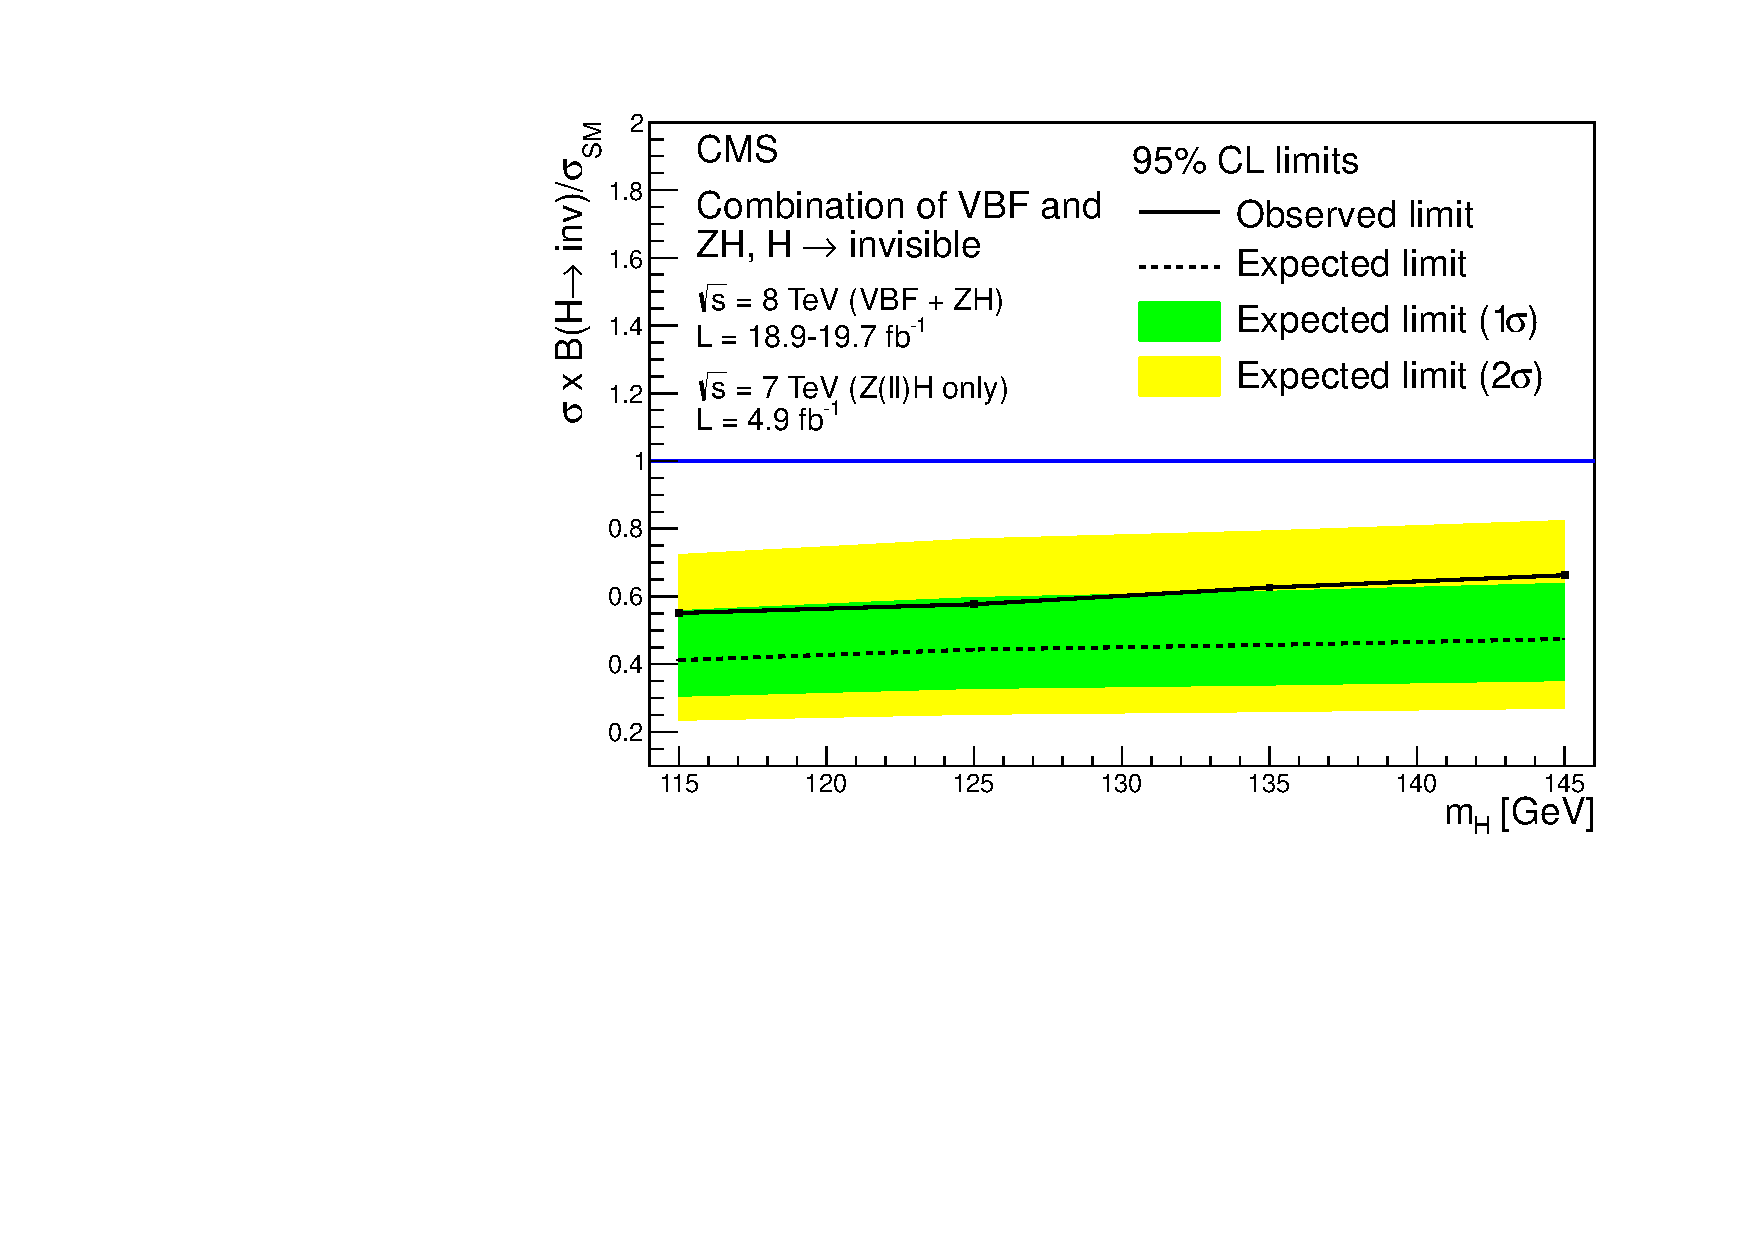
\includegraphics[width=\largefigwidth]{plots/prompt/HIG-13-30-figs/combinedlimit.pdf}
  \caption{Expected and observed 95\% \ac{CL} upper limits on the $\sigma\times\BRinv/\sigma_{SM}$ obtained from the combination of the \ac{VBF}, Z$(\ell\ell)$H and Z$(b\bar{b})$H searches. The green and yellow bands indicate the 68\% and 95\% confidence intervals on the expected limit respectively~\cite{Chatrchyan:2014tja}.}
  \label{fig:promptcomb}
\end{figure}

\begin{figure}
  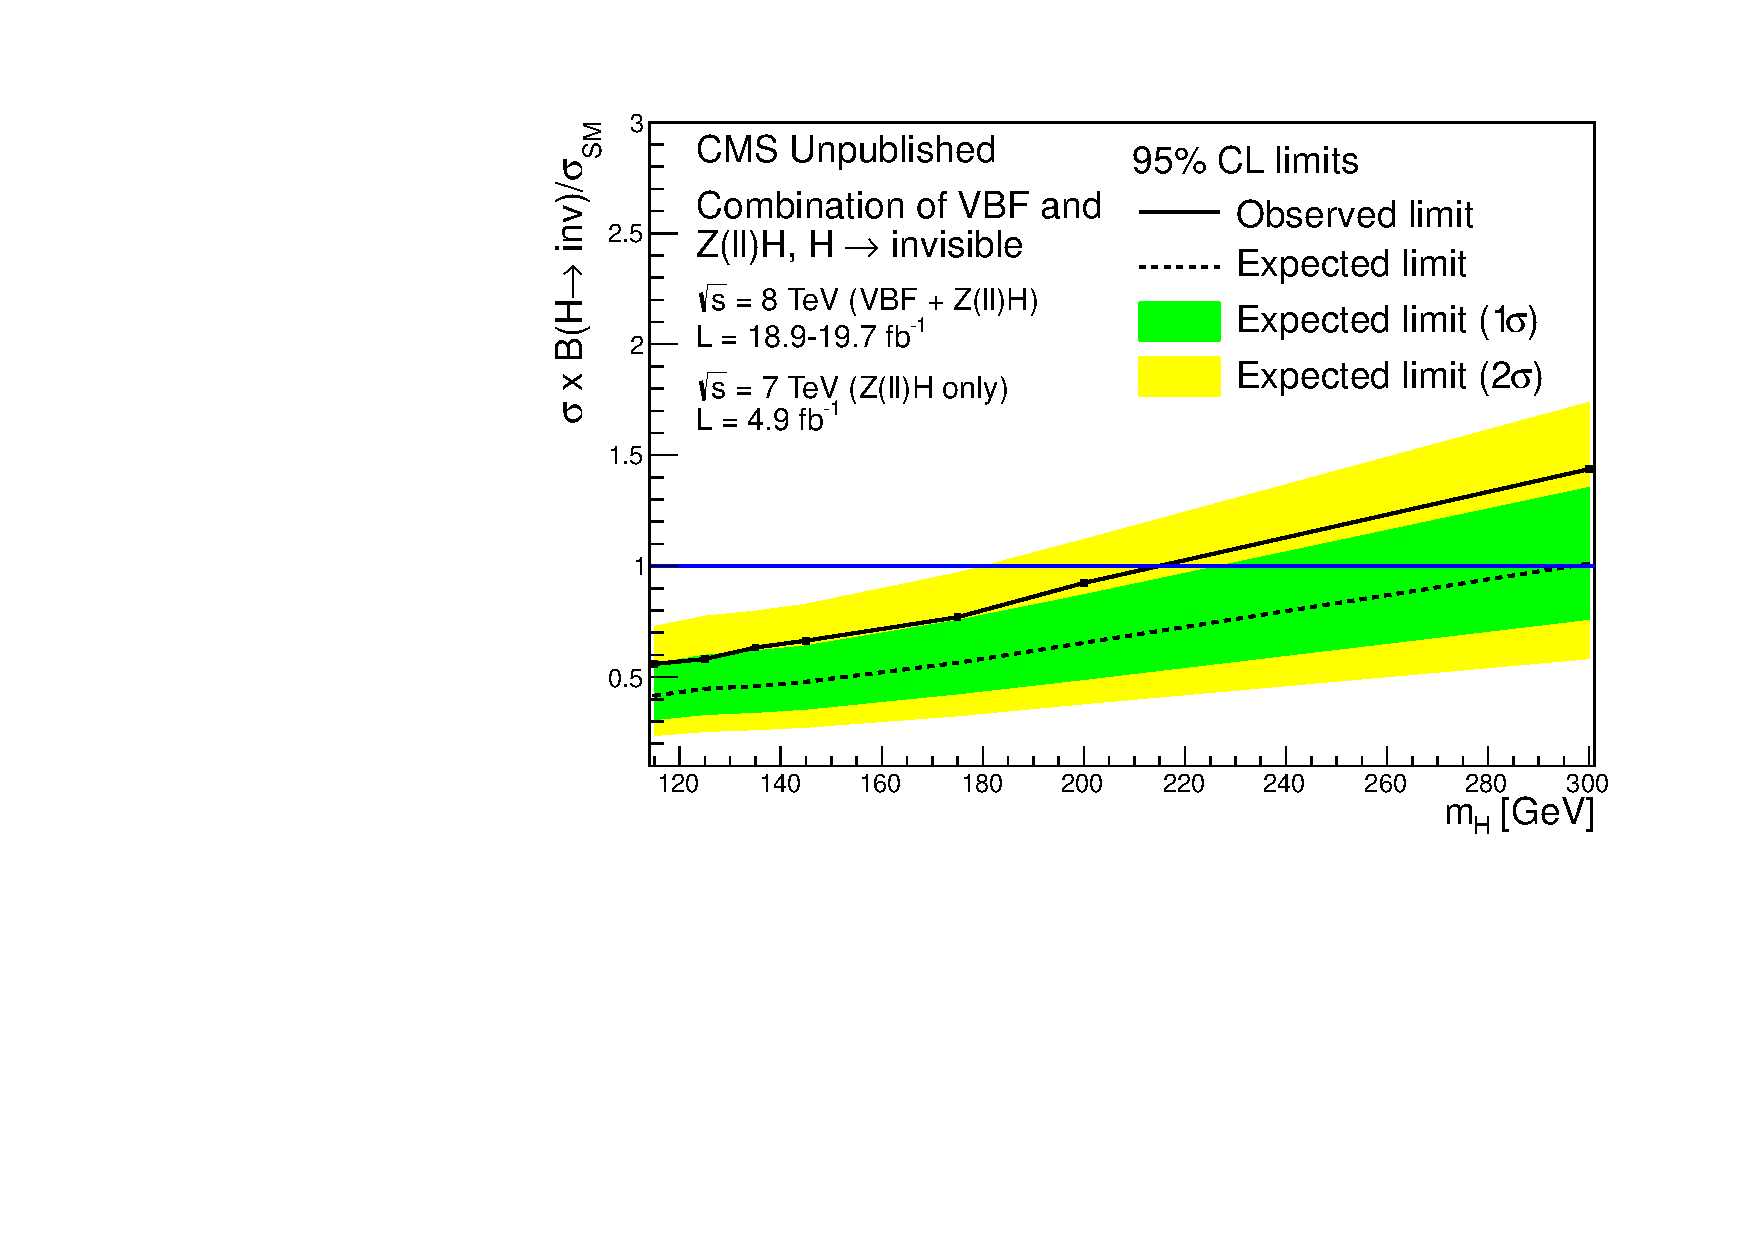
\includegraphics[width=\largefigwidth]{plots/prompt/HIG-13-30-figs/highmasslimit.pdf}
  \caption{Expected and observed 95\% \ac{CL} upper limits on the $\sigma\times\BRinv/\sigma_{SM}$ obtained from the combination of the \ac{VBF} and Z$(\ell\ell)$H searches. The green and yellow bands indicate the 68\% and 95\% confidence intervals on the expected limit respectively~\cite{Chatrchyan:2014tja}.}
  \label{fig:promptcombhighmass}
\end{figure}

\section{Combination with the parked data VBF search}
\label{sec:combparked}
%Present combination
The parked data \ac{VBF} analysis was combined with both the ZH searches and the monojet search, which was finished in 2015~\cite{CMS-PAS-HIG-15-012}. The prompt data \ac{VBF} analysis was not included in this combination due to its large overlap with the parked data analysis. As discussed above, overlaps between the \ac{VBF} and monojet searches were explicitly removed by vetoing events in the monojet search passing the \ac{VBF} selection. The resolved category of the monojet search was also removed from the combination to avoid large overlap with the Z$(b\bar{b})$H search. This removal did not change the expected limit, as the resolved category is the least sensitive to invisibly decaying Higgs bosons. The remaining overlaps between the monojet search and the ZH searches are small as discussed in \SectionRef{sec:monojet}.

%syst studies, correlation of JES,JER and why met scale in monojet not correlated why zbbH as above
After resolving the issue of overlaps, it was necessary to study which uncertainties were correlated. A summary of the correlated uncertainties, and the analyses they affect is given in \TableRef{tab:parkedcorrs}. Of particular note are the decisions taken in correlating the jet and \MET uncertainties. For the jet uncertainties, as in the combination with the \ac{VBF} prompt data analysis, the uncertainties on the jet energy in the Z($b\bar{b})$H analysis are not correlated with the other analyses due to the very different method of determining the jet energy. In the remaining three analyses, the \ac{JES} and \ac{JER} uncertainties vary as a function of a jet's \pt and $\eta$, so it is important to study the jet kinematic distributions when deciding which of the uncertainties should be correlated. As described in \SectionRef{sec:monojet}, the two categories of the monojet search used in this combination require very high \pt jets which are mostly in the central region of the detector. By contrast the high \pt jets in the \ac{VBF} parked data analysis are mostly in the forward region of the detector due to the large \detajj requirement. The Z$(\ell\ell)$H analysis uses low \pt jets with \pt$>30$ \GeV similar to those used to calculate \jetmetdphi in the \ac{VBF} analysis, but very different from the high \pt central jets in the monojet analysis. The decision was therefore taken to correlate the \ac{VBF} and Z$(\ell\ell)$H analyses \ac{JES} and \ac{JER} uncertainties and to leave those from the monojet analysis uncorrelated. A study of the impact of this choices was carried out, and it was found that all combinations of correlations resulted in the same expected limit.

In the case of the \MET uncertainties, the two ZH searches and the \ac{VBF} search use the same \MET corrections, whereas the monojet search applies a different set of corrections~\cite{CMS-PAS-EXO-12-055}. The monojet analysis \ac{UES} uncertainty was therefore not correlated with that from the other analyses.

\begin{table}
  \caption{Uncertainties correlated between the \ac{VBF} parked data, Z$(\ell\ell)$H, Z$(b\bar{b})$H and monojet searches and the analyses they affect.}
  \label{tab:parkedcorrs}
  \begin{tabular}{|l|c|}
      \hline
      Nuisance & Analyses which it affects \\
      \hline
      \ac{JES} & VBF, Z($\ell\ell$)H \\
      PDFs & VBF, Z($b\bar{b}$), Z($\ell\ell$)H, monojet \\
      QCD scale & VBF, Z($b\bar{b}$), Z($\ell\ell$)H, monojet \\
      Luminosity & VBF, Z($b\bar{b}$)H, Z($\ell\ell$)H, monojet \\
      \ac{JER} & VBF, Z($\ell\ell$)H \\
      \ac{UES} & VBF, Z($b\bar{b}$)H, Z($\ell\ell$)H \\
      Muon identification efficiency & VBF, Z($\ell\ell$)H, monojet \\
      Electron identification efficiency & VBF, Z($\ell\ell$)H \\
      Diboson cross-section & VBF, monojet \\
      \hline
    \end{tabular}
\end{table}

%combination results and explain by channel
With these uncertainty correlations the four searches were combined for a Higgs boson mass of 125 \GeV assuming \ac{SM} production-cross-sections for each channel. The 95\% \ac{CL} observed (expected) limit on \BRinv for a 125 \GeV Higgs boson was found to be 0.36 (0.30). The log-likelihood obtained as a function of \BRinv is shown in \FigureRef{fig:parkedcombscan}. The favoured observed value can be seen to be greater than zero, however this is not significant.

\begin{figure}
  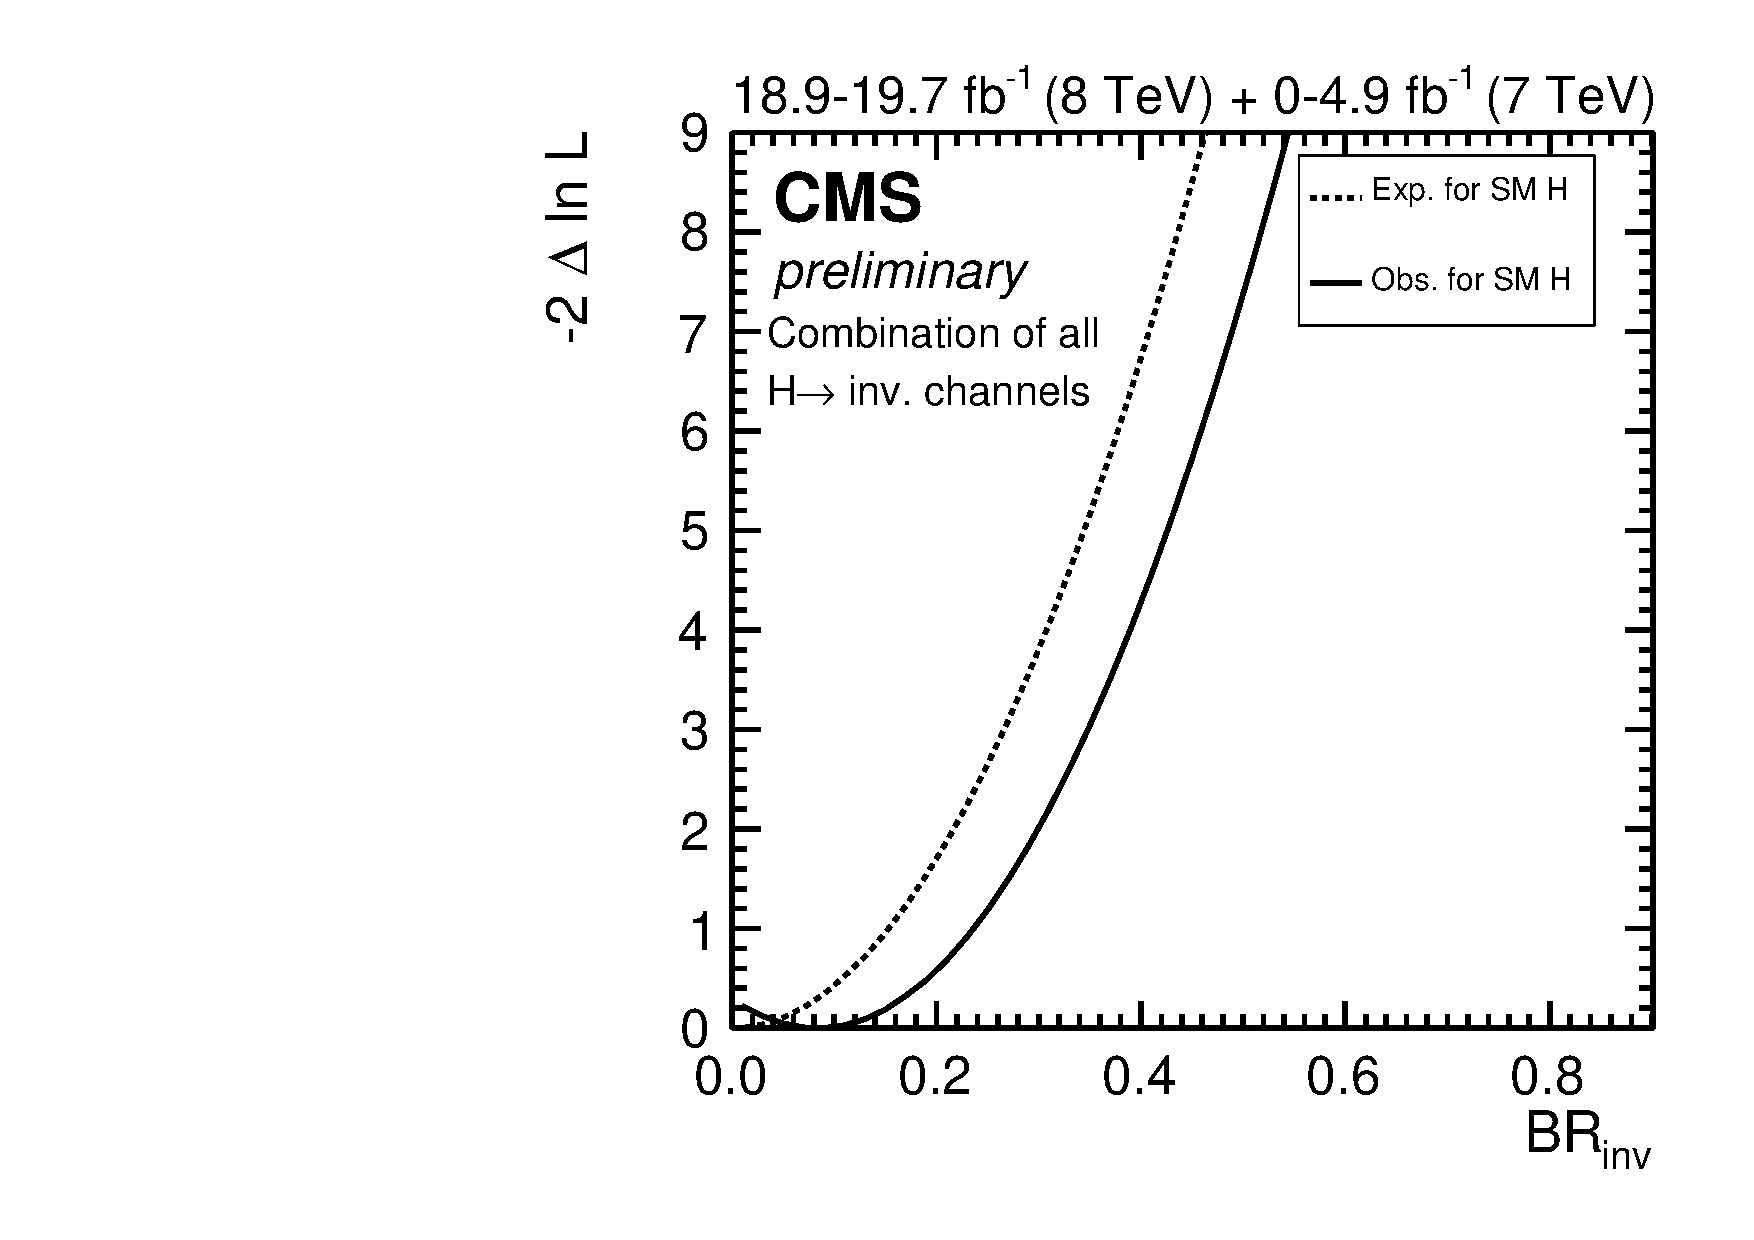
\includegraphics[width=\largefigwidth]{plots/comb/HIG-15-012-figs/combscan.pdf}
  \caption{Log-likelihood versus \BRinv. The solid curve represents the observation in data and the dashed curves represent the median expected result for no invisible decays of the Higgs boson~\cite{CMS-PAS-HIG-15-012}.}
  \label{fig:parkedcombscan}
\end{figure}

As well as the full combination of all analysis categories, sub-combinations were also performed of all the categories targeting a particular production mode. The results of these sub-combinations and the full combination is shown in \FigureRef{fig:parkedcombchannel}, where the \ac{VBF}-tagged limit comes from the \ac{VBF} parked data analysis, the \ac{VH}-tagged limit from the resolved category of the monojet analysis and the two ZH searches, and the \ac{ggH} tagged limit comes from the monojet category of the monojet analysis. It can be seen that whilst the \ac{VBF} channel is the most sensitive, the limits, are improved significantly by the addition of the analyses targeting the two other production modes.

\begin{figure}
  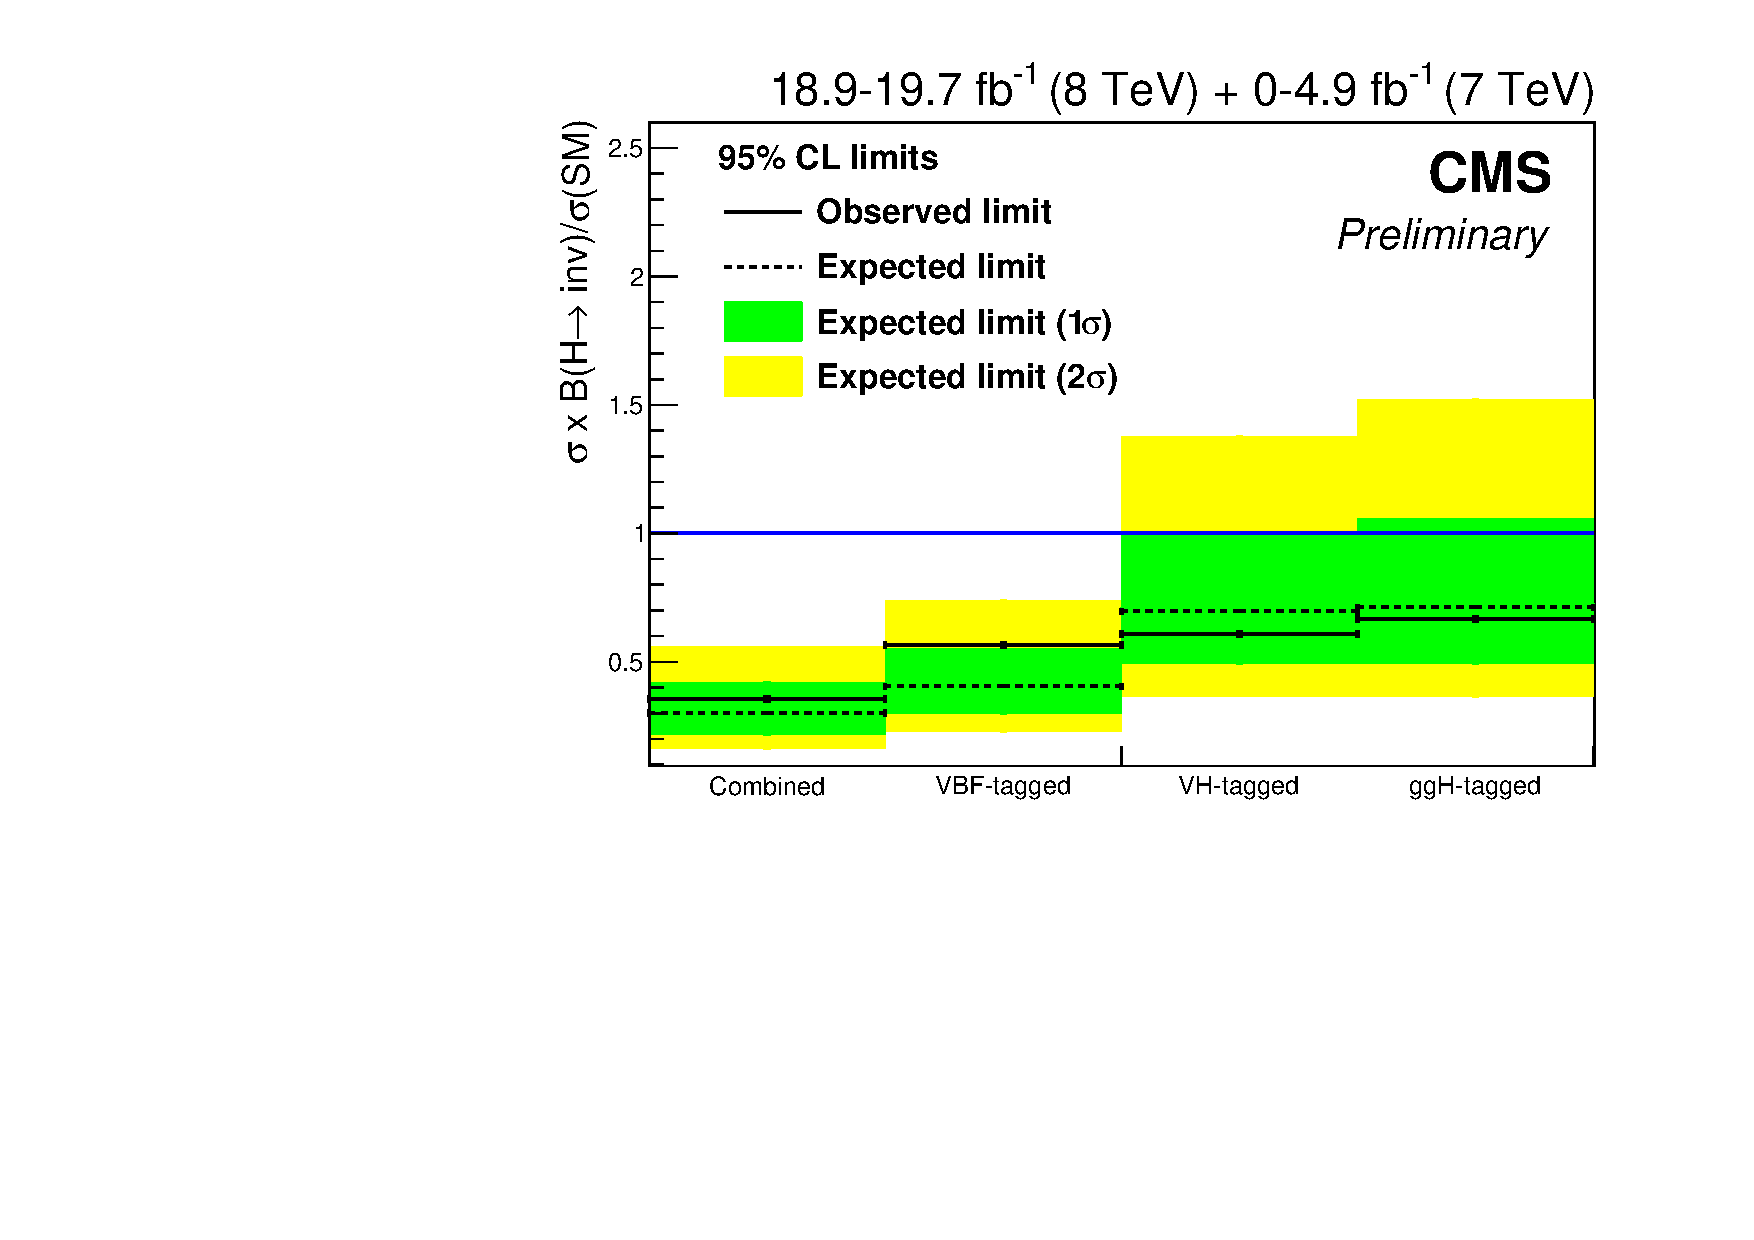
\includegraphics[width=\largefigwidth]{plots/comb/HIG-15-012-figs/channellimit.pdf}
  \caption{Expected and observed 95\% \ac{CL} upper limits on production cross-section times \BRinv normalised to the \ac{SM} production cross-section obtained from the combination of all channels targeting each Higgs boson production mode. The green and yellow bands indicate the 68\% and 95\% confidence intervals on the expected limit respectively~\cite{CMS-PAS-HIG-15-012}.}
  \label{fig:parkedcombchannel}
\end{figure}

%??conclusion
